\documentclass[a4paper,12pt]{article}
\usepackage{amsmath, amsthm, amsfonts, amssymb}
\usepackage{microtype}
\usepackage{geometry}
\usepackage{booktabs}
\usepackage{graphicx}
\usepackage{caption}
\usepackage{subcaption}
% \geometry{margin=1in}

\newtheoremstyle{exerciseStyle}
{ } % Space above
{ } % Space below
{ \normalfont } % Body font
{ } % Indent amount
{ \bfseries } % Theorem head font
{ } % Punctuation after theorem head
{ } % Space after theorem head
{ \thmname{#1}\thmnumber{ #2} } % Theorem head spec (can be left empty, meaning `normal`)
\theoremstyle{exerciseStyle}
\newtheorem{exercise}{Exercise}[section]

\newtheoremstyle{solutionStyle}
{ } % Space above
{ } % Space below
{ \normalfont } % Body font
{ } % Indent amount
{ \bfseries } % Theorem head font
{ } % Punctuation after theorem head
{ } % Space after theorem head
{ \thmname{#1}\thmnumber{ #2} } % Theorem head spec (can be left empty, meaning `normal`)
\theoremstyle{solutionStyle}
\newtheorem{solution}{Solution}[section]

\title{
    MEK4250\\
    \small{Exercises for Finite Elements in Computational Mechanics}
}
\author{August Femtehjell}
\date{January 24, 2025}

\begin{document}

\maketitle

\tableofcontents

\section{Elliptic equations and the finite element method}

\section{A glimpse at the finite element method}

\begin{exercise}
    Consider the problem $-u''(x) = x^2$ on the unit interval with $u(0) = u(1) = 0$.
    Let $u = \sum_{k = 1}^N u_k \sin{(\pi k x)}$ and $v = \sin{(\pi l x)}$ for $l = 1, \ldots, N$, for e.g.\ $N = 10, 20, 40$ and solve $(1.9)$.
    What is the error in $L_2$ and $L_\infty$.
\end{exercise}

\begin{solution}
    In this exercise, we use the Galerkin method to solve the problem, wishing to solve the problem as $Au = b$, where
    \begin{align*}
        A_{ij} &= \int_\Omega k \nabla N_j \cdot \nabla N_i \, dx, \\
        b_i &= \int_\Omega f N_i \, dx + \int_{\partial \Omega_N} h N_i \, ds.
    \end{align*}
    We begin by noting that
    \begin{equation*}
        \nabla N_i = \frac{d}{dx} \sin{(\pi i x)} = \pi i \cos{(\pi i x)},
    \end{equation*}
    such that
    \begin{align*}
        \int_\Omega k \nabla N_j \cdot \nabla N_i \, dx
        = \int_0^1 k \pi^2 i j \cos{(\pi j x)} \cos{(\pi i x)} \, dx
        = \frac{\pi^2 i^2}{2} \delta_{ij}.
    \end{align*}

    As we are given that the Dirichlet boundary conditions cover the entire boundary, and $\partial \Omega_D \cap \partial \Omega_N = \emptyset$, we have that the Neumann boundary integral is zero.
    The $b$ vector is then given by
    \begin{align*}
        b_i &= \int_\Omega f N_i \, dx
        = \int_0^1 x^2 \sin{(\pi i x)} \, dx
        = \frac{(2 - \pi^2 i^2)(-1)^i- 2}{\pi^3 i^3}.
    \end{align*}

    Setting up and solving the system for varying $N$ is then rather simples, implemented in \verb|1_elliptic/ex1.py|.
    This gives the errors presented in Table~\ref{tab:1_1}, with the plotted solution in Figure~\ref{fig:1_1_curve}.
    \begin{table}[!ht]
        \caption{Errors of approximations of $u$ for varying $N$, with sine basis functions.\label{tab:1_1}}
        \centering
        \begin{tabular}{lrr}
            \toprule
            $N$ & $L_2$ & $L_\infty$ \\
            \midrule
            10 & 0.001791 & 0.000224 \\
            20 & 0.000338 & 0.000059 \\
            40 & 0.000062 & 0.000015 \\
            \bottomrule
        \end{tabular}
    \end{table}

    \begin{figure}[!ht]
        \centering
        \begin{subfigure}[b]{0.45\textwidth}
            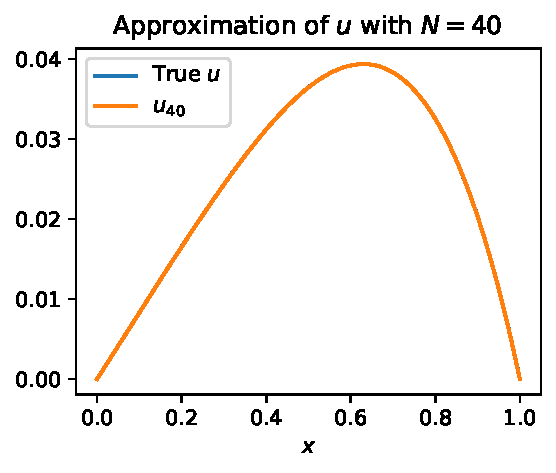
\includegraphics[width=\textwidth]{1_elliptic/exercise_1_1.pdf}
            \caption{Approximated function.\label{fig:1_1_curve}}
        \end{subfigure}
        \hfill
        \begin{subfigure}[b]{0.45\textwidth}
            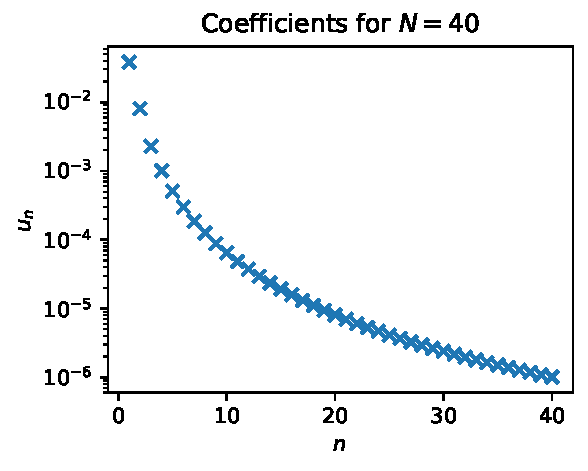
\includegraphics[width=\textwidth]{1_elliptic/exercise_1_1_coeffs.pdf}
            \caption{Coefficients $|u_k|$.\label{fig:1_1_coeffs}}
        \end{subfigure}
        % 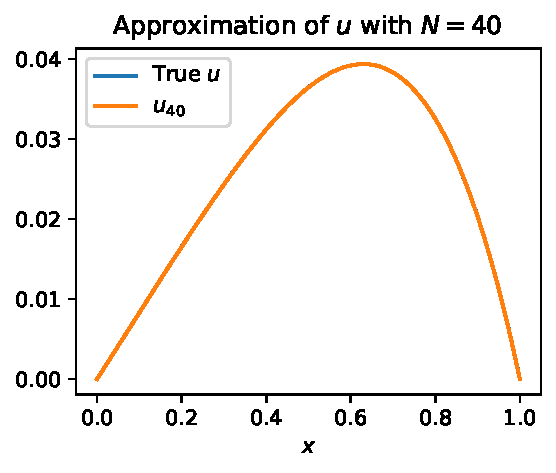
\includegraphics[width=0.7\textwidth]{1_elliptic/exercise_1_1.pdf}
        \caption{Approximation of $u$ with $N = 40$ sine basis functions.\label{fig:1_1}}
    \end{figure}
\end{solution}

\begin{exercise}
    Consider the same problem as in the previous exercise, but using the Bernstein polynomials.
    That is, the basis for the Bernstein polynomial of order $N$ on the unit inteval is $B_k^N(x) = x^k (1 - x)^{N - k}$ for $k = 0, \ldots, N$.
    Let $u = \sum_{k = 0}^N u_k B_k^N(x)$ and $v = B_l^N(x)$ for $l = 0, \ldots, N$ and solve $(1.9)$.
    What is the error in $L_2$ and $L_\infty$ in terms of $N$ for $N = 1, 2, \ldots, 10$.
    Remark: Do the basis functions satisfy the boundary condtions? Should some of them be removed?
\end{exercise}

\begin{solution}
    The Bernstein polynomials $B_0^N$ and $B_N^N$ both need to be removed, as they do not satisfy the Dirichlet boundary conditions, as $B_0^N(0)  = 1 = B_N^N(1)$.
    We therefore need atleast $N = 3$, in order to get an atleast somewhat viable solution.

    The Bernstein basis polynomials are defined as
    \begin{equation*}
        B_k^N(x) = \binom{N}{k} x^k (1 - x)^{N - k}.
    \end{equation*}
    Some useful properties which might come in handy are
    \begin{enumerate}
        \item The derivative of a basis polynomials is
            \begin{equation*}
                \left( B_k^N(x) \right)' = N \left( B_{k-1}^{N-1}(x) - B_{k}^{n-1}(x) \right),
            \end{equation*}
            where we follow the convention of setting $B_{-1}^N(x) = 0 = B_{N+1}^N(x)$.

        \item The definite integral on the unit line is given by
            \begin{equation*}
                \int_0^1 B_{k}^N(x) = \frac{1}{N+1} \quad \text{for } k = 0, 1, \ldots, N.
            \end{equation*}

        \item The multiple of two Bernstein polynomials is
            \begin{align*}
                B_k^N(x) \cdot B_q^M(x) &= \binom{N}{k} x^k (1 - x)^{N - k} \binom{M}{q} x^q (1 - x)^{M - q} \\
                &= \binom{N}{k} \binom{M}{q} x^{k+q} (1 - x)^{N + M - k - q} \\
                &= \frac{\binom{N}{k}\binom{M}{q}}{\binom{N + M}{k + q}} B_{k+q}^{N + M}(x)
            \end{align*}
    \end{enumerate}

    From these, we can gather that
    \begin{equation*}
        \int_{0}^{1} B_k^N(x) B_q^M(x) \ dx = \frac{\binom{N}{k}\binom{M}{q}}{\binom{N + M}{k + q}} \int_0^1 B_{k+q}^{N + M}(x) \ dx = \frac{\binom{N}{k}\binom{M}{q}}{(N + M + 1) \binom{N + M}{k + q}}.
    \end{equation*}
    The terms in the stiffness matrix are then given by
    \begin{align*}
        A_{ij} &= \int_{0}^{1} \nabla B_i^N(x) \cdot \nabla B_{j}^N(x) \ dx \\
        &= N^2 \int_{0}^{1} \left( B_{i-1}^{N - 1} - B_{i}^{N - 1} \right) \left( B_{j-1}^{N - 1} - B_{j}^{N - 1} \right) \ dx \\
        &= N^2
        \int_{0}^{1} B_{i-1}^{N - 1} B_{j-1}^{N - 1}
        - B_{i}^{N - 1} B_{j-1}^{N - 1}
        - B_{i-1}^{N - 1} B_{j}^{N - 1}
        + B_{i}^{N - 1} B_{j}^{N - 1} \ dx
        \\
        &= N^2 \int_{0}^{1} \alpha_{i-1, j-1} B_{i+j-2}^{2N-2} - (\alpha_{i,j-1} + \alpha_{i-1, j}) B_{i+j-1}^{2N - 2} + \alpha_{i,j} B_{i+j}^{2N - 2} \ dx \\
        &= \frac{N^2}{2N - 1} \left(
            \frac{\binom{N-1}{i-1}\binom{N-1}{j-1}}{\binom{2N - 2}{i + j - 2}}
            - \frac{
                \binom{N-1}{i}\binom{N-1}{j-1}
                + \binom{N-1}{i-1}\binom{N-1}{j}
            }{\binom{2N - 2}{i + j - 1}}
            + \frac{\binom{N-1}{i}\binom{N-1}{j}}{\binom{2N - 2}{i + j}}
        \right)
    \end{align*}
    This can likely be written much nicer, however I cannot be bothered to do that right now.

    Opting to take the easy way out instead, and utilizing \verb|sympy| to solve the integrals, we can implement the solution in \verb|1_elliptic/ex2.py|.
    The errors are presented in Table~\ref{tab:1_2}.
    As we can read from the table, the polynomial approximation is exact for $N > 3$, which is expected as the Bernstein polynomials are exact for polynomials of degree $N$.

    \begin{table}[!ht]
        \centering
        \caption{Errors of approximations of $u$ for varying $N$, with Bernstein basis functions.\label{tab:1_2}}
        \begin{tabular}{cc}
            \toprule
            $N$ & $L_2$ \\
            \midrule
            2 & $\frac{\sqrt{1330}}{6300}$ \\
            3 & $\frac{\sqrt{70}}{12600}$ \\
            4--10 & 0 \\
            \bottomrule
        \end{tabular}
    \end{table}
\end{solution}

\begin{exercise}
    Consider the same problem as in the previous exercise, but with $ -u''(x) = \sin(k\pi x)$ for $k = 1$ and $k = 10$.
\end{exercise}

\begin{solution}
    The approach for this is approximately the same, however we need to figure out the true solution in order to calculate the error.
    \begin{align*}
        u''(x) &= -\sin(k\pi x) \\
        u'(x) &= \frac{1}{k\pi} \cos(k\pi x) + C_1 \\
        u(x) &= \frac{1}{k^2\pi^2} \sin(k\pi x) + C_1 x + C_2.
    \end{align*}
    As we have Dirichlet boundary conditions, we then set $C_1 = 0 = C_2$.
\end{solution}

\begin{exercise}
    Consider the same problem as in the previous exercise, but with the finite element method in for example FEniCS, FEniCSx or Firedrake, using Lagrange method of order 1, 2 and 3.
\end{exercise}

\begin{solution}
    For this exercise, I will be using FEniCSx to solve the problem.
    The code is implemented in \verb|doc/1_elliptic/ex4.py|, with the resulting approximations in Figure~\ref{fig:ex4}.
    \begin{figure}
        \centering
        \begin{subfigure}[b]{0.45\textwidth}
            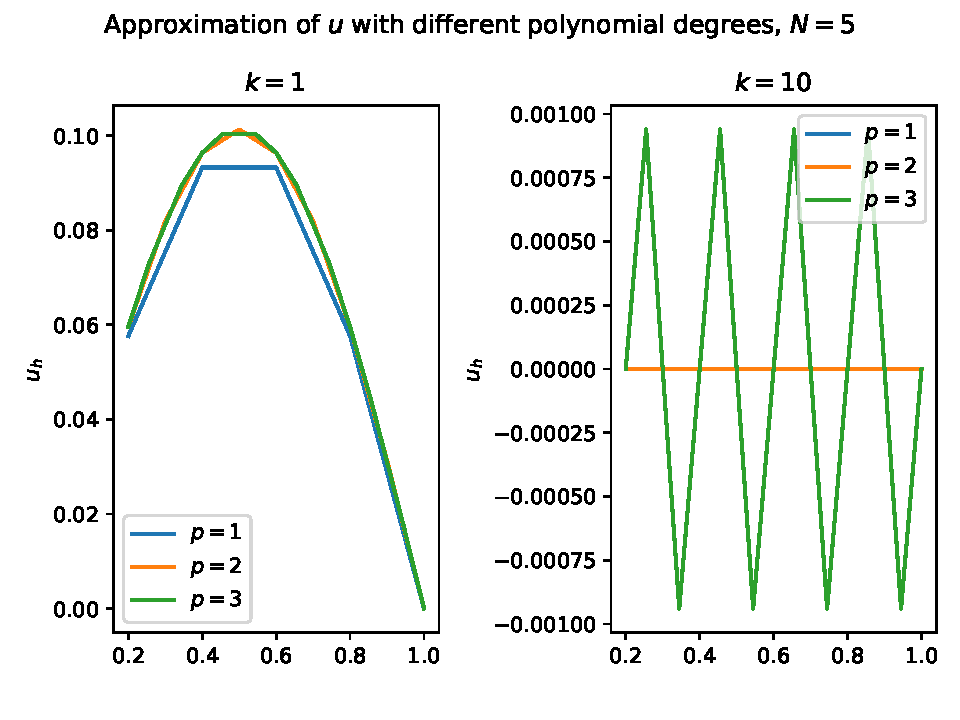
\includegraphics[width=\textwidth]{1_elliptic/exercise_1_4_N=5.pdf}
            \caption{$N=5$.\label{fig:ex4_1}}
        \end{subfigure}
        \hfill
        \begin{subfigure}[b]{0.45\textwidth}
            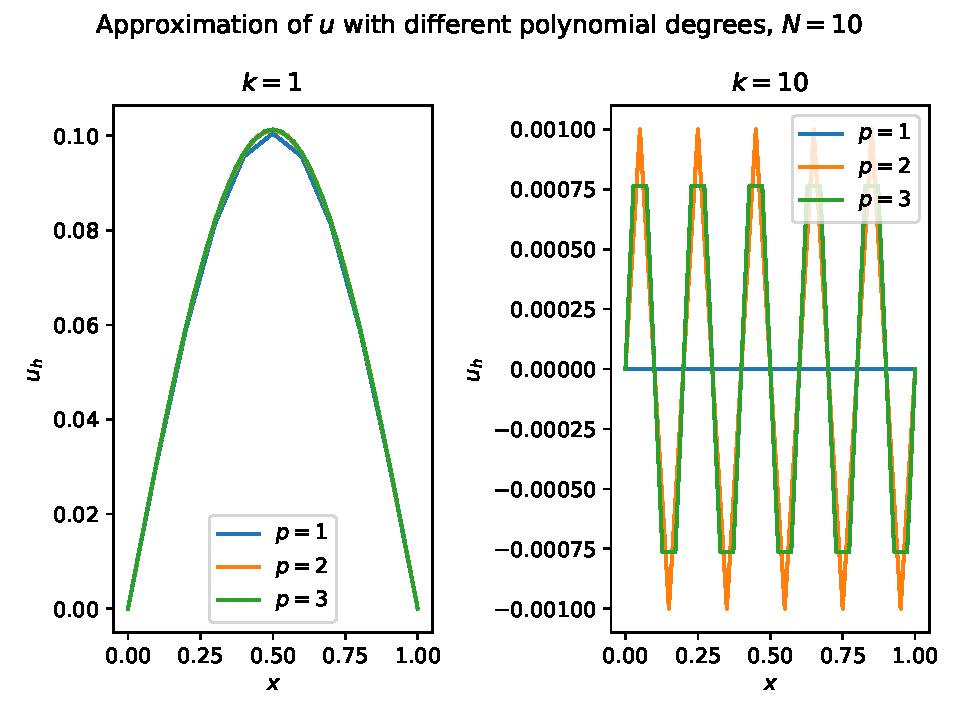
\includegraphics[width=\textwidth]{1_elliptic/exercise_1_4_N=10.pdf}
            \caption{$N=10$.\label{fig:ex4_2}}
        \end{subfigure}
        \begin{subfigure}[b]{0.45\textwidth}
            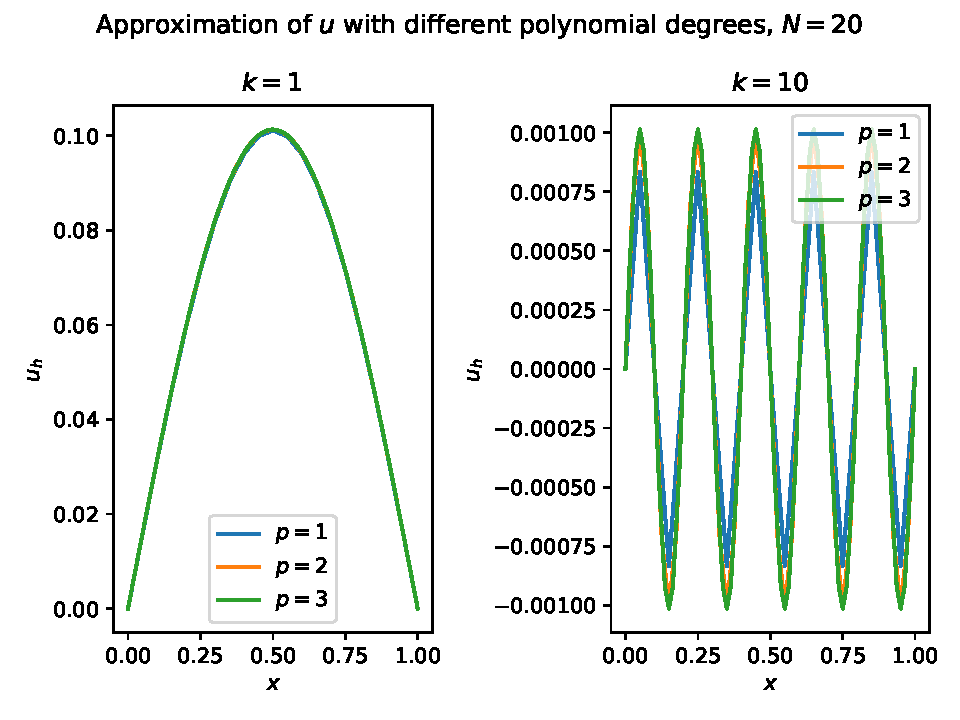
\includegraphics[width=\textwidth]{1_elliptic/exercise_1_4_N=20.pdf}
            \caption{$N=20$.\label{fig:ex4_3}}
        \end{subfigure}
        \hfill
        \begin{subfigure}[b]{0.45\textwidth}
            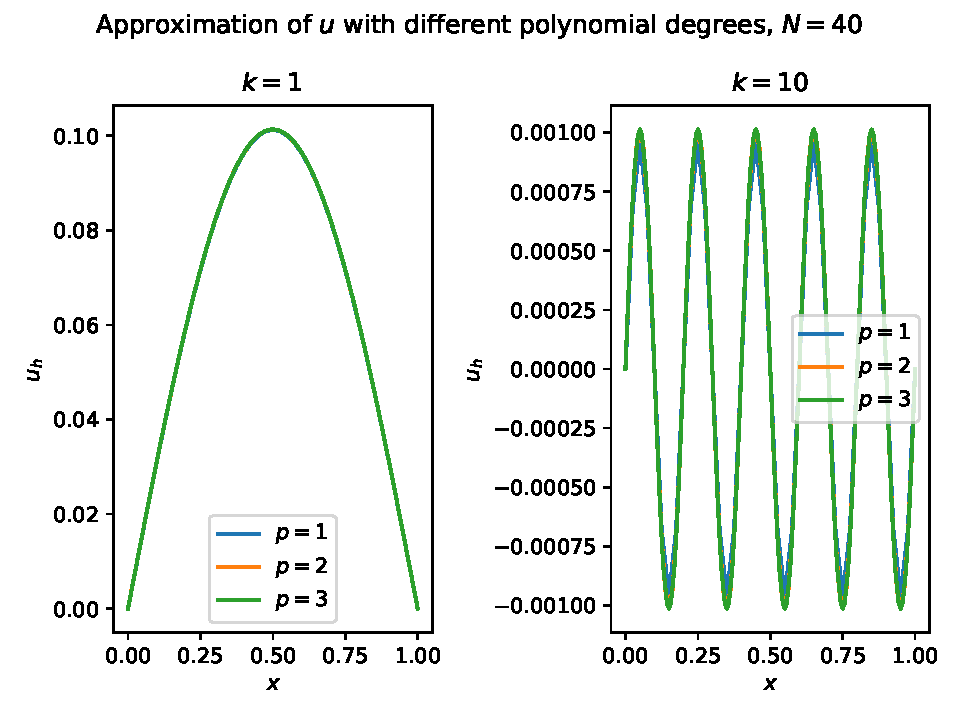
\includegraphics[width=\textwidth]{1_elliptic/exercise_1_4_N=40.pdf}
            \caption{$N=40$.\label{fig:ex4_4}}
        \end{subfigure}
        \caption{Approximation of $u$ with varying $N$ elements.\label{fig:ex4}}
    \end{figure}
\end{solution}

\end{document}